\documentclass{article}
\author{Lena Morrill}
\date{\today}
\title{Transcriptomic analysis of the organoids}

\usepackage{tikz}
\usepackage{lscape}
\usepackage{array}
\usepackage{graphicx}
\usepackage{hyperref}

\setlength{\textwidth}{6.7in}
\setlength{\oddsidemargin}{-0.1in}
\setlength{\textheight}{8.6in}
\setlength{\topmargin}{-0.4in}

\def\checkmark{\tikz\fill[scale=0.4](0,.35) -- (.25,0) -- (1,.7) -- (.25,.15) -- cycle;} 
\newcolumntype{L}[1]{>{\raggedright\let\newline\\\arraybackslash\hspace{0pt}}m{#1}}
\newcolumntype{C}[1]{>{\centering\let\newline\\\arraybackslash\hspace{0pt}}m{#1}}
\newcolumntype{R}[1]{>{\raggedleft\let\newline\\\arraybackslash\hspace{0pt}}m{#1}}


\begin{document}
\maketitle

\tableofcontents

\section{Data}
\subsection{3' bias}

Three RNASeq samples -- PDO14, PDO16, and PDO18 -- have a clear 3' bias. Three others -- PDO4, PDO13, PDO17 -- have a slighy bias. Only the first three have been removed from the analyses.

\subsection{Summary of organoids}
See table below.

% latex table generated in R 4.0.3 by xtable 1.8-4 package
% Fri Mar 12 11:30:34 2021

\begin{landscape}

\begin{table}[ht]
{ \scriptsize
\centering
\begin{tabular}{rL{.4in}L{.3in}L{.3in}L{.3in}R{.3in}L{.1in}L{.1in}L{.3in}llL{.2in}L{.3in}L{.2in}L{.3in}L{.15in}L{.15in}L{.2in}L{.2in}L{.2in}L{.3in}L{.3in}L{.3in}}
  \hline
 & PDO & ID & sWGS & RNAseq & OVO4& & Cor. CN-GE & Comments & scDNA? & S4 & WGD & CCNE1 amp & CCNE1 amp (RNA or CN) & Chromotripsis & Tandem dup & \#segments & Ploidy & Quiet & Change from ascites & CDK12 amp & CDK12 loss & Chemonaive \\ 
  \hline
1 & PDO1 & 151723 & 19844 & 19938 & 920.00 &  & Y & Very similar to PDO11 &  & \checkmark & \checkmark &  &  &  &  & Very low & Very high &  & ? & $\times$ & $\times$ & \checkmark \\ 
  2 & PDO11 & 54327 & 118976 & 19905 & 413.00 &  & N & Very similar to PDO1 &  &  & &  & \checkmark &  &  & Very low & Med &  & $\times$ & $\times$ & $\times$ & $\times$ \\ 
  3 & PDO10 & 119178 & 119127 & 19907 & 788.00 &  & N &  &  & \checkmark &  &  &  &  &  & Med & Med &  & ? & $\times$ & $\times$ & $\times$ \\ 
  4 & PDO13 & 54276 & 19846 & 19940 & 297.00 &  & Y &  &  &  &  &  &  &  &  & Med & Med &  & ? & \checkmark & $\times$ & $\times$ \\ 
  5 & PDO15 & 118947 & 54327 & 19904 & 333.00 &  & N &  &  & \checkmark &  &  &  &  &  & Med & Med &  & $\times$ & $\times$ & $\times$ & $\times$ \\ 
  6 & PDO17 & 50495 & 50495- & 19916 & 348.00 &  & Y &  &  & \checkmark &  &  &  &  &  & Med & Med &  & ? & $\times$ & $\times$ & $\times$ \\ 
  7 & PDO18 & 32070 & 32070- & 19920 & 47.00 &  & - &  &  & \checkmark &  &  &  &  &  & Low & Med &  & ? & $\times$ & $\times$ & $\times$ \\ 
  8 & PDO2 & 23868 & jb95a- & 19917 & 75.00 &  & Y &  & \checkmark & \checkmark &  & \checkmark & \checkmark &  &  & Med & Med &  & ? & $\times$ & $\times$ & $\times$ \\ 
  9 & PDO3 & 118976 & 119178 & 19906 & 466.00 &  & N &  & \checkmark & \checkmark &  &  & \checkmark & \checkmark &  & Med & Med &  & $\times$ & $\times$ & $\times$ & $\times$ \\ 
  10 & PDO9 & 119058 & 119058- & 19921 & 466.00 &  & Y &  &  & \checkmark &  &  &  & (!) surely also has tandem duplication? &  & Med & Med &  & ? & $\times$ & $\times$ & $\times$ \\ 
  11 & PDO14 & 54288 & 19829 & 19925 & 409.00 &  & - &  &  & \checkmark &  &  & \checkmark &  &  & High & Med &  & $\times$ & \checkmark & $\times$ & $\times$ \\ 
  12 & PDO4 & 151773 & 19848 & 19942 & 571.00 &  & Y &  &  & \checkmark &  &  & \checkmark &  & \checkmark & Very high & Med &  & ? & $\times$ & $\times$ & $\times$ \\ 
  13 & PDO5 & 119127 & 118947 & 19903 & 627.00 &  & N &  &  & \checkmark &  &  &  &  &  & Med & Med &  & ? & $\times$ & $\times$ & $\times$ \\ 
  14 & PDO6 & 119148 & 119148 & 19902 & 627.00 &  & Y &  & \checkmark & \checkmark &  &  &  &  &  & Med & Med &  & ? & $\times$ & $\times$ & $\times$ \\ 
  15 & PDO16 & 119025 & 19842 & 19936 & 839.00 &  & - &  &  &  &  &  &  &  &  & Low & Low & \checkmark & $\times$ & $\times$ & \checkmark & $\times$ \\ 
  16 & PDO12 & 151761 & 19845 & 19939 & 467.00 &  & Y &  &  &  &  &  &  &  &  & Low & Low & \checkmark & \checkmark & $\times$ & \checkmark & $\times$ \\ 
  17 & PDO7 & 32077 & 19847 & 19941 & 366.00 &  & Y &  &  &  &  &  &  &  &  & Low & Low & \checkmark & ? & $\times$ & $\times$ & $\times$ \\ 
  18 & PDO8 & 54059 & 19843 & 19937 & 366.00 &  & Y &  &  &  &  &  &  &  &  & Low & Low & \checkmark & ? & $\times$ & $\times$ & $\times$ \\ 
%  19 & FT1 & fal01 &  & 19950 &  &  &  &  &  &  &  &  &  &  &  &  &  &  &  &  &  &  \\ 
%  20 & FT10 & fal10 &  & 19953 &  &  &  &  &  &  &  &  &  &  &  &  &  &  &  &  &  &  \\ 
%  21 & FT7 & fal07 &  & 19952 &  &  &  &  &  &  &  &  &  &  &  &  &  &  &  &  &  &  \\ 
%  22 & FT7-bis & fal07 &  & 19954 &  &  &  &  &  &  &  &  &  &  &  &  &  &  &  &  &  &  \\ 
%  23 & FT8 & fal08 &  & 19955 &  &  &  &  &  &  &  &  &  &  &  &  &  &  &  &  &  &  \\ 
%  24 & FT9 & fal09 &  & 19951 &  &  &  &  &  &  &  &  &  &  &  &  &  &  &  &  &  &  \\ 
   \hline
\end{tabular}
}
\end{table}

\end{landscape}

\section{Transcriptomics of organoids}
The PCA including all organoids (first plot) shows a split in PC1 between the three samples of high 3' bias and the rest. PC2 splits the three samples with slightly high samples from the rest. Once the top 3' bias samples have been removed (second plot), PC2 of the first plot becomes PC1.

\begin{figure}[h]
\centering
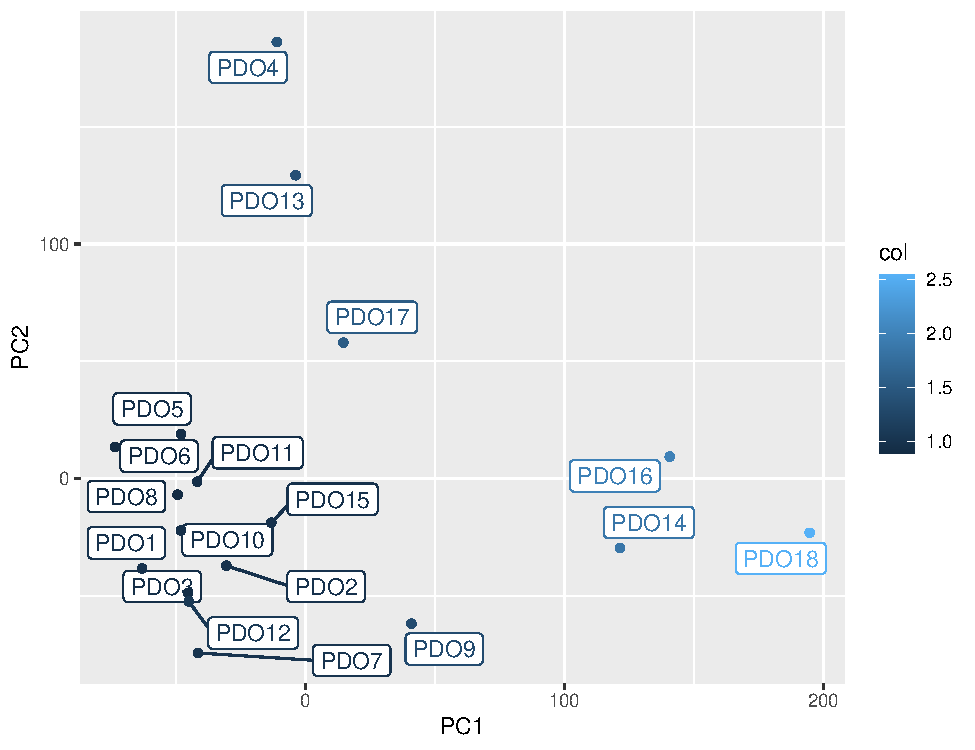
\includegraphics[width=3.2in]{../../RNASeq_DE_resistant_sensitive/figures/PCA_RNASeq/3primebias_PCA_counts.pdf}
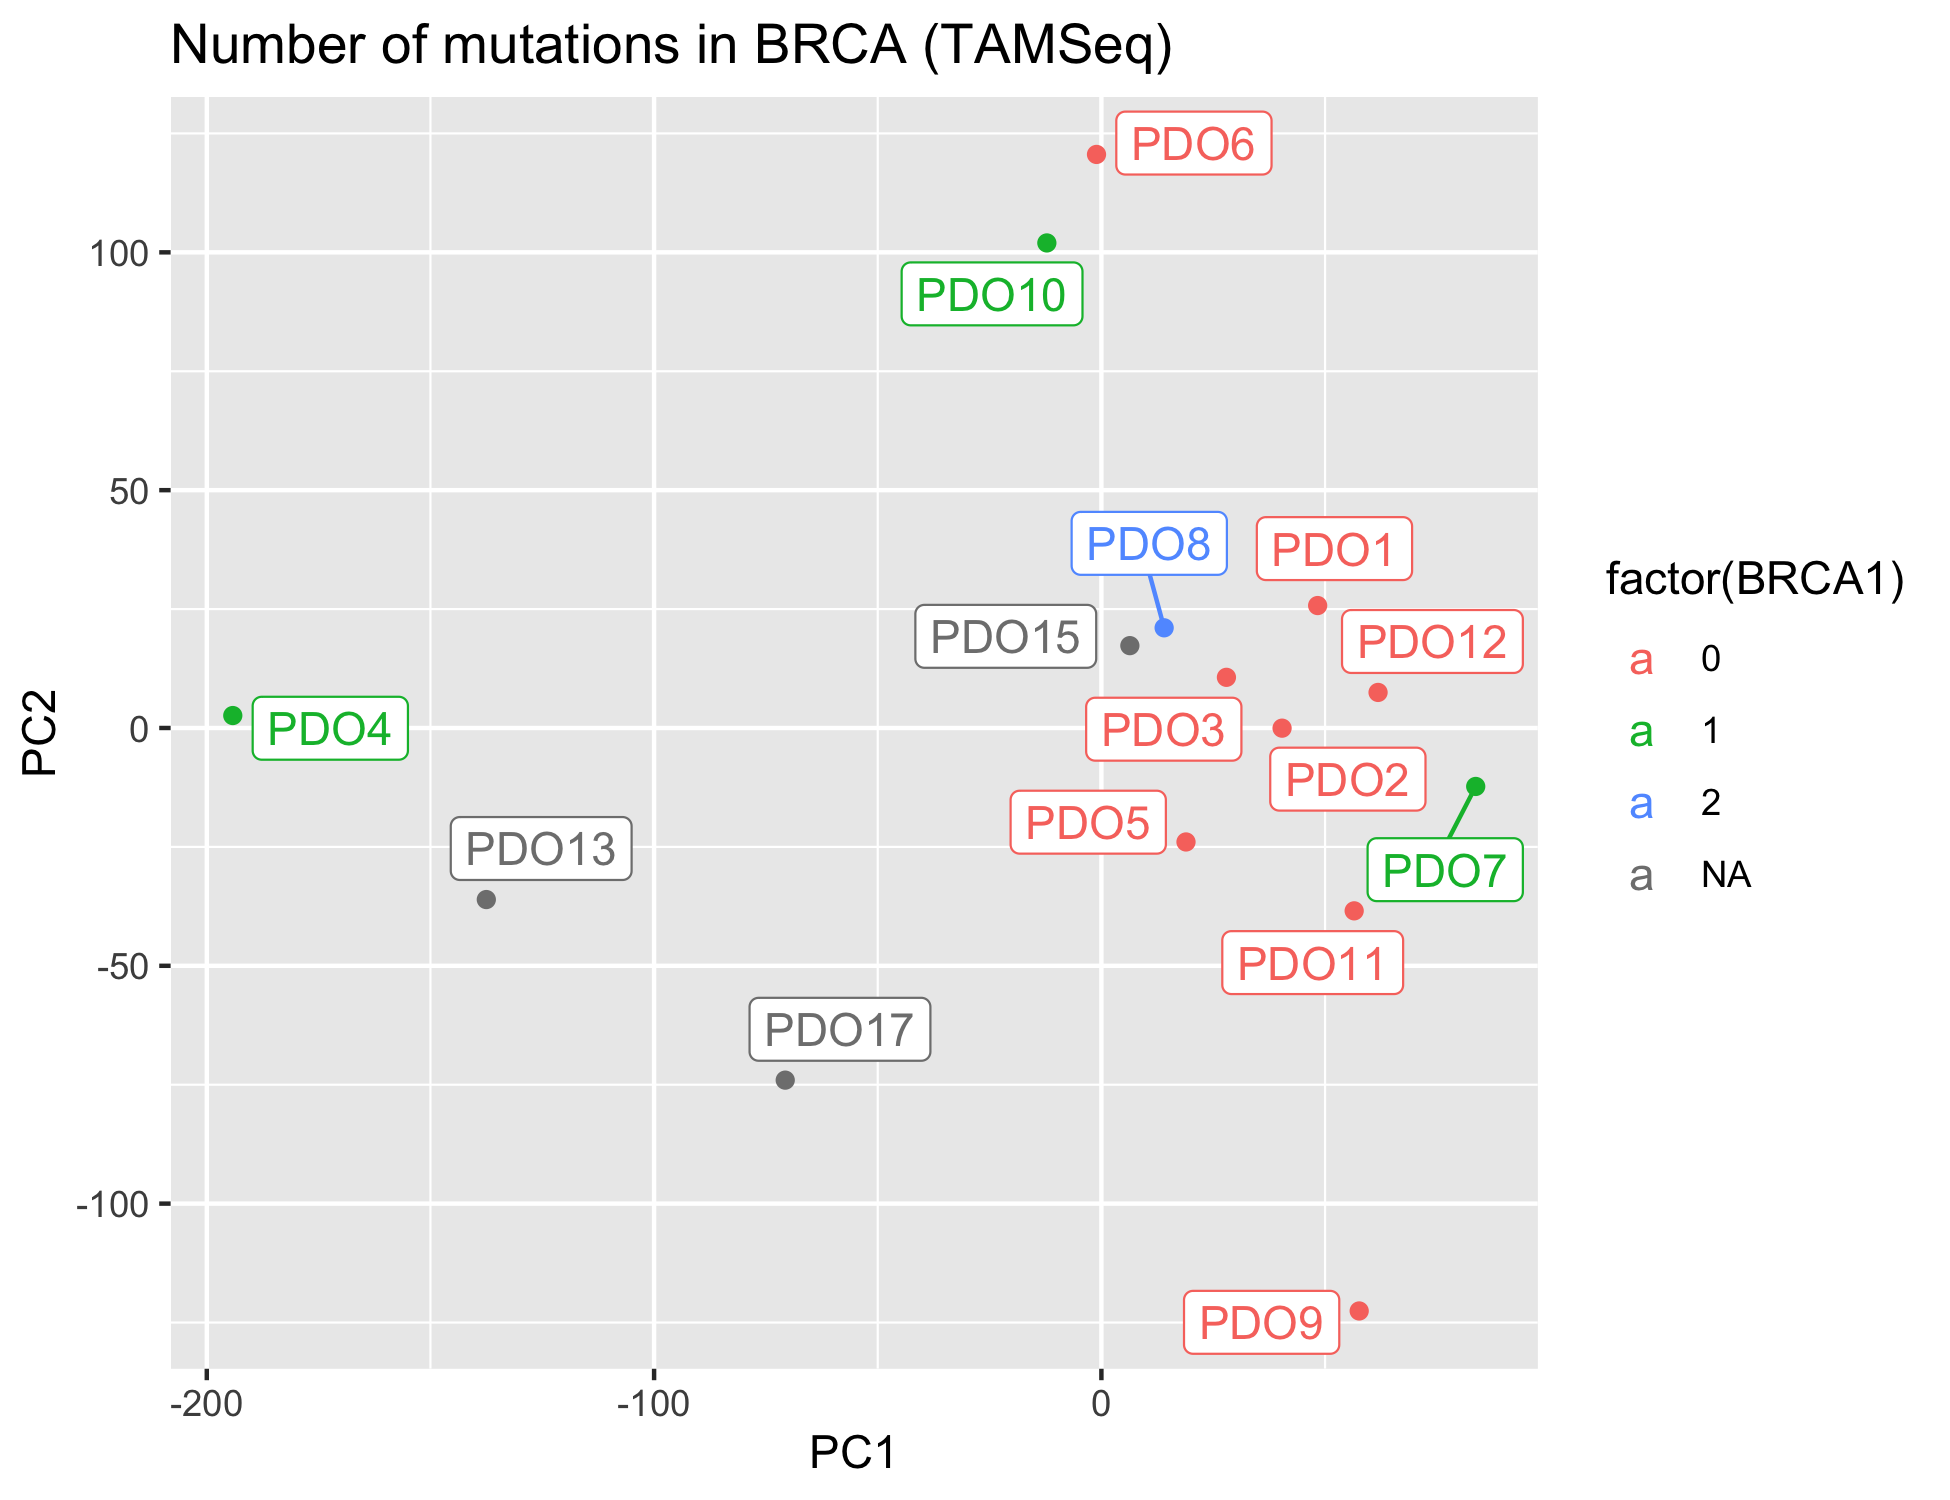
\includegraphics[width=3.4in]{../../RNASeq_DE_resistant_sensitive/figures/PCA_RNASeq/PCA_counts_subset_BRCA_TAMSeq.png}
\caption{PCA including all samples (left) and only the ones without 3' bias (right; colour coded by number of mutations in BRCA).}
\end{figure}

\subsection{Organoids $vs$ normal ovarian tissue DE}

\begin{center} \emph{Done by Stephane} \end{center}

\subsection{Sensitive organoids $vs$ resistant organoids DE}
\begin{center} \emph{Done by Stephane} \end{center}


\clearpage
\subsection{Comparison with TCGA}

We compare the average gene expression values (in DESeq2 counts, but the results are similar for TPM=transcripts per million transcripts) between 240 TCGA samples and 15 organoids (see first plot of Figure~\ref{tcga_org_cor_rnaseq}), for 33610 genes. The second plot shows the TPM of TCGA samples (violin plots) and organoids (red points), for genes of interest. We can see there is a good agreement between the two, althoug there is a slight bias for organoid samples to have higher TPM values. This could be explained by  organoids containing pure tumour populations -- since TPMs are compositional data, low expression of genes expressed in the TME can lead to high expression values of the rest of genes (amongst them, the ones included here).

\begin{figure}[h]
\centering
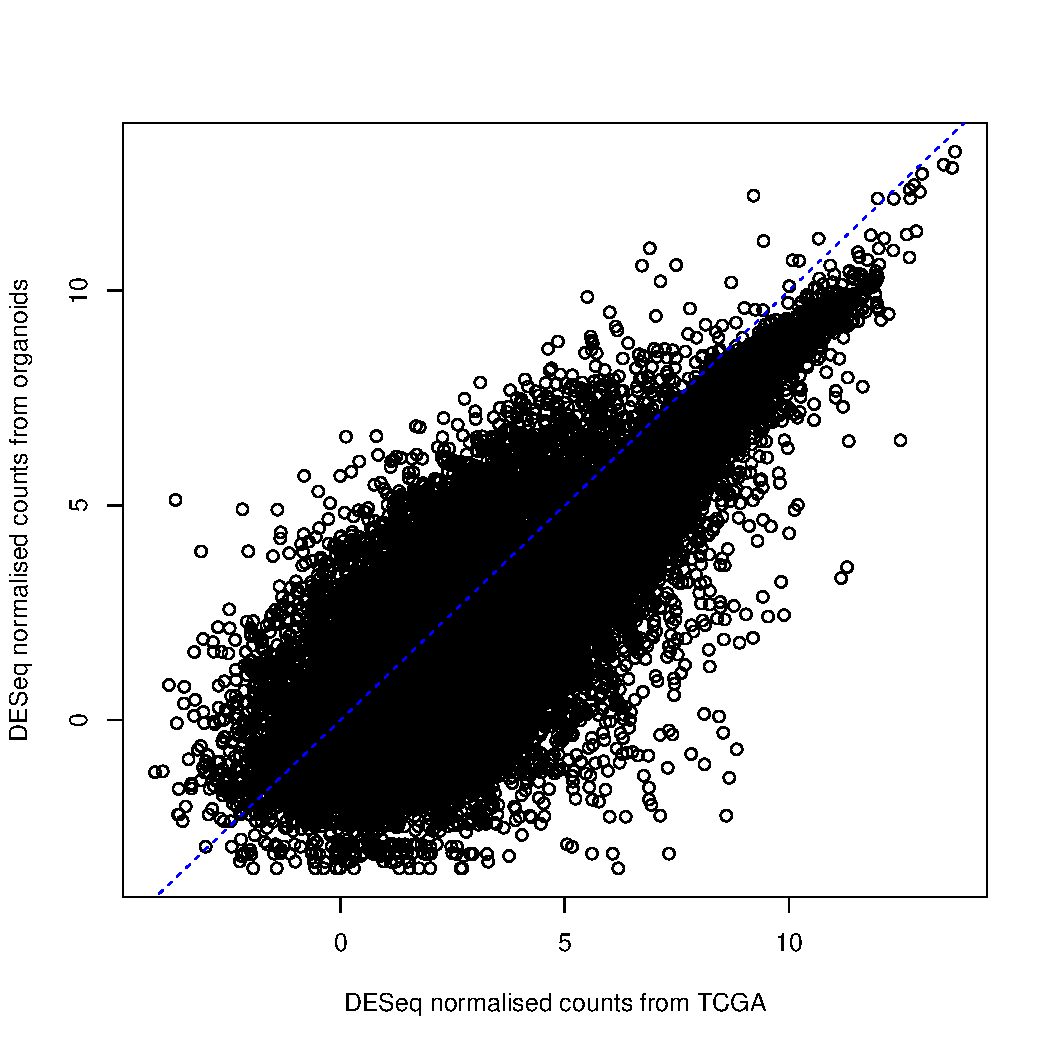
\includegraphics[width=.42\textwidth]{../../RNASeq_DE_resistant_sensitive/figures/Sensitive_resistant_figures/colmeans_deseqcounts_correlation_tcga_org.pdf}
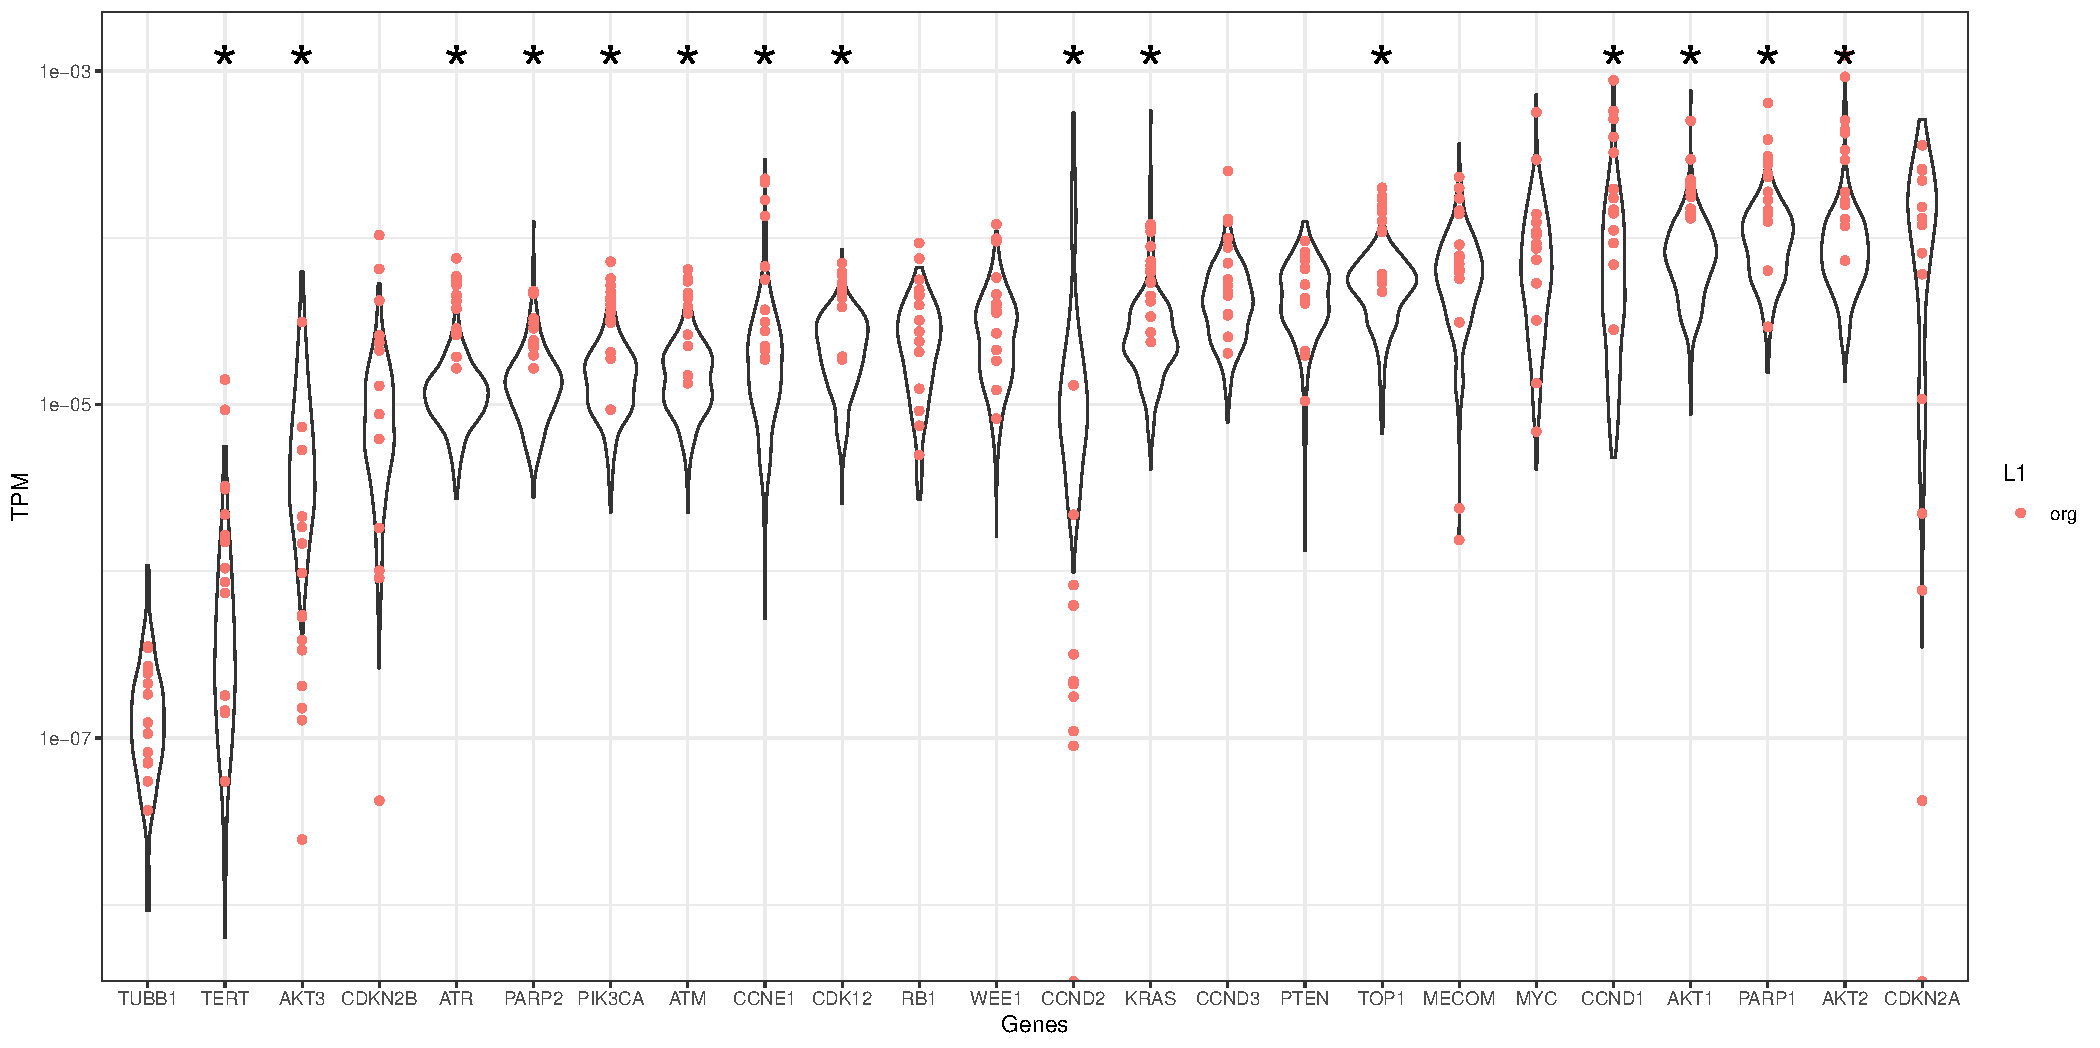
\includegraphics[width=\textwidth]{../../RNASeq_DE_resistant_sensitive/figures/Sensitive_resistant_figures/TPM_correlation_tcga_org_selected_genes.pdf}
\caption{TPM for genes of interest in organoids (points) and in TCGA (violin plots). Genes which have a different distribution according to a Kolmogorov-Smirnov test are marked with an asterisk.\label{tcga_org_cor_rnaseq}}
\end{figure}

\clearpage

\subsection{(Resistant $vs$ sensitive in organoids) $vs$ (complete remission or response $vs$ progressive disease in TCGA) }

There is an extremely bad correlation for both log2 fold changes and $p$-values. As we don't expect to find a perfect match anyway (as (1) progressive disease would work as a surrogate for resistant, but there are many more factors and (2) it's an organoid comparison $vs$ a primary tissue comparison) we have not pursued this further.

\section{Correlation of gene expression (GE) and copy number (CN)}

\subsection{Genome-wide correlations}
There are two values for gene expression that we can work with:
\begin{itemize}
\item (Computed by Lena) the weighted average copy number value per gene
\item (Computed by Stephane) the copy number value is assigned to each gene which is the closest to a copy number area of high variability (variability computed as the variance across samples)
\end{itemize}

In the genes of interest (MYC, etc.) the two are almost always the same (meaning that the relevant copy number segment is on the gene). The conclusions from Stephane's analysis is that there were some correlations in certain genes, but that they were mostly driven by only a couple of organoids (!). 

\medskip

In my analysis there were some extreme copy number values that were excluded as outliers -- they all belong to the samples 118976org or 119058org, that come from the same patient. There is no obvious correlation between raw CN values and counts (TPM or DESeq2), either pooling all organoids or doing an organoid-specific scatterplot (See Figures \href{https://github.com/lm687/Organoids_Compositional_Analysis/blob/master/RNASeq_and_CN/figures/joint_counts_CN_DESeq_all.pdf}{[scatterplot per organoid DESeq2]} and \href{https://github.com/lm687/Organoids_Compositional_Analysis/blob/master/RNASeq_and_CN/figures/joint_counts_CN_TPM_all.pdf}{[scatterplot per organoid TPM]}).

\medskip

This prompted us to scale the CN and GE values (scaled between organoids to a mean of zero and a standard deviation of 1). This gives a much better correlation, especially when segments of copy number of two are excluded from the analysis (see \ref{fig:scaled_CN_GE}). However, it seems as though this trend only applies to some organoids. Organoids PDO11, PDO10, PDO15, PDO3, PDO5 show no trend between GE and CN. These organoids don't have anything special when it comes to exposures, and they are not the ones with relatively high 3' bias.

\medskip

A similar approach is to compare the ranks of the organoids in CN and GE (see Figure~\ref{fig:rank_CN_GE}).

\medskip

A couple of important considerations are: gene expression values are correlated (only slightly, but this can become important in whole genome analyses), and copy number regions can be extremely large, making the link between copy number and any gene tenuous. There are some further correlations imposed on the data once you scale them, but I don't think this can explain the difference in trends between organoids.

\begin{figure}[h]
\centering
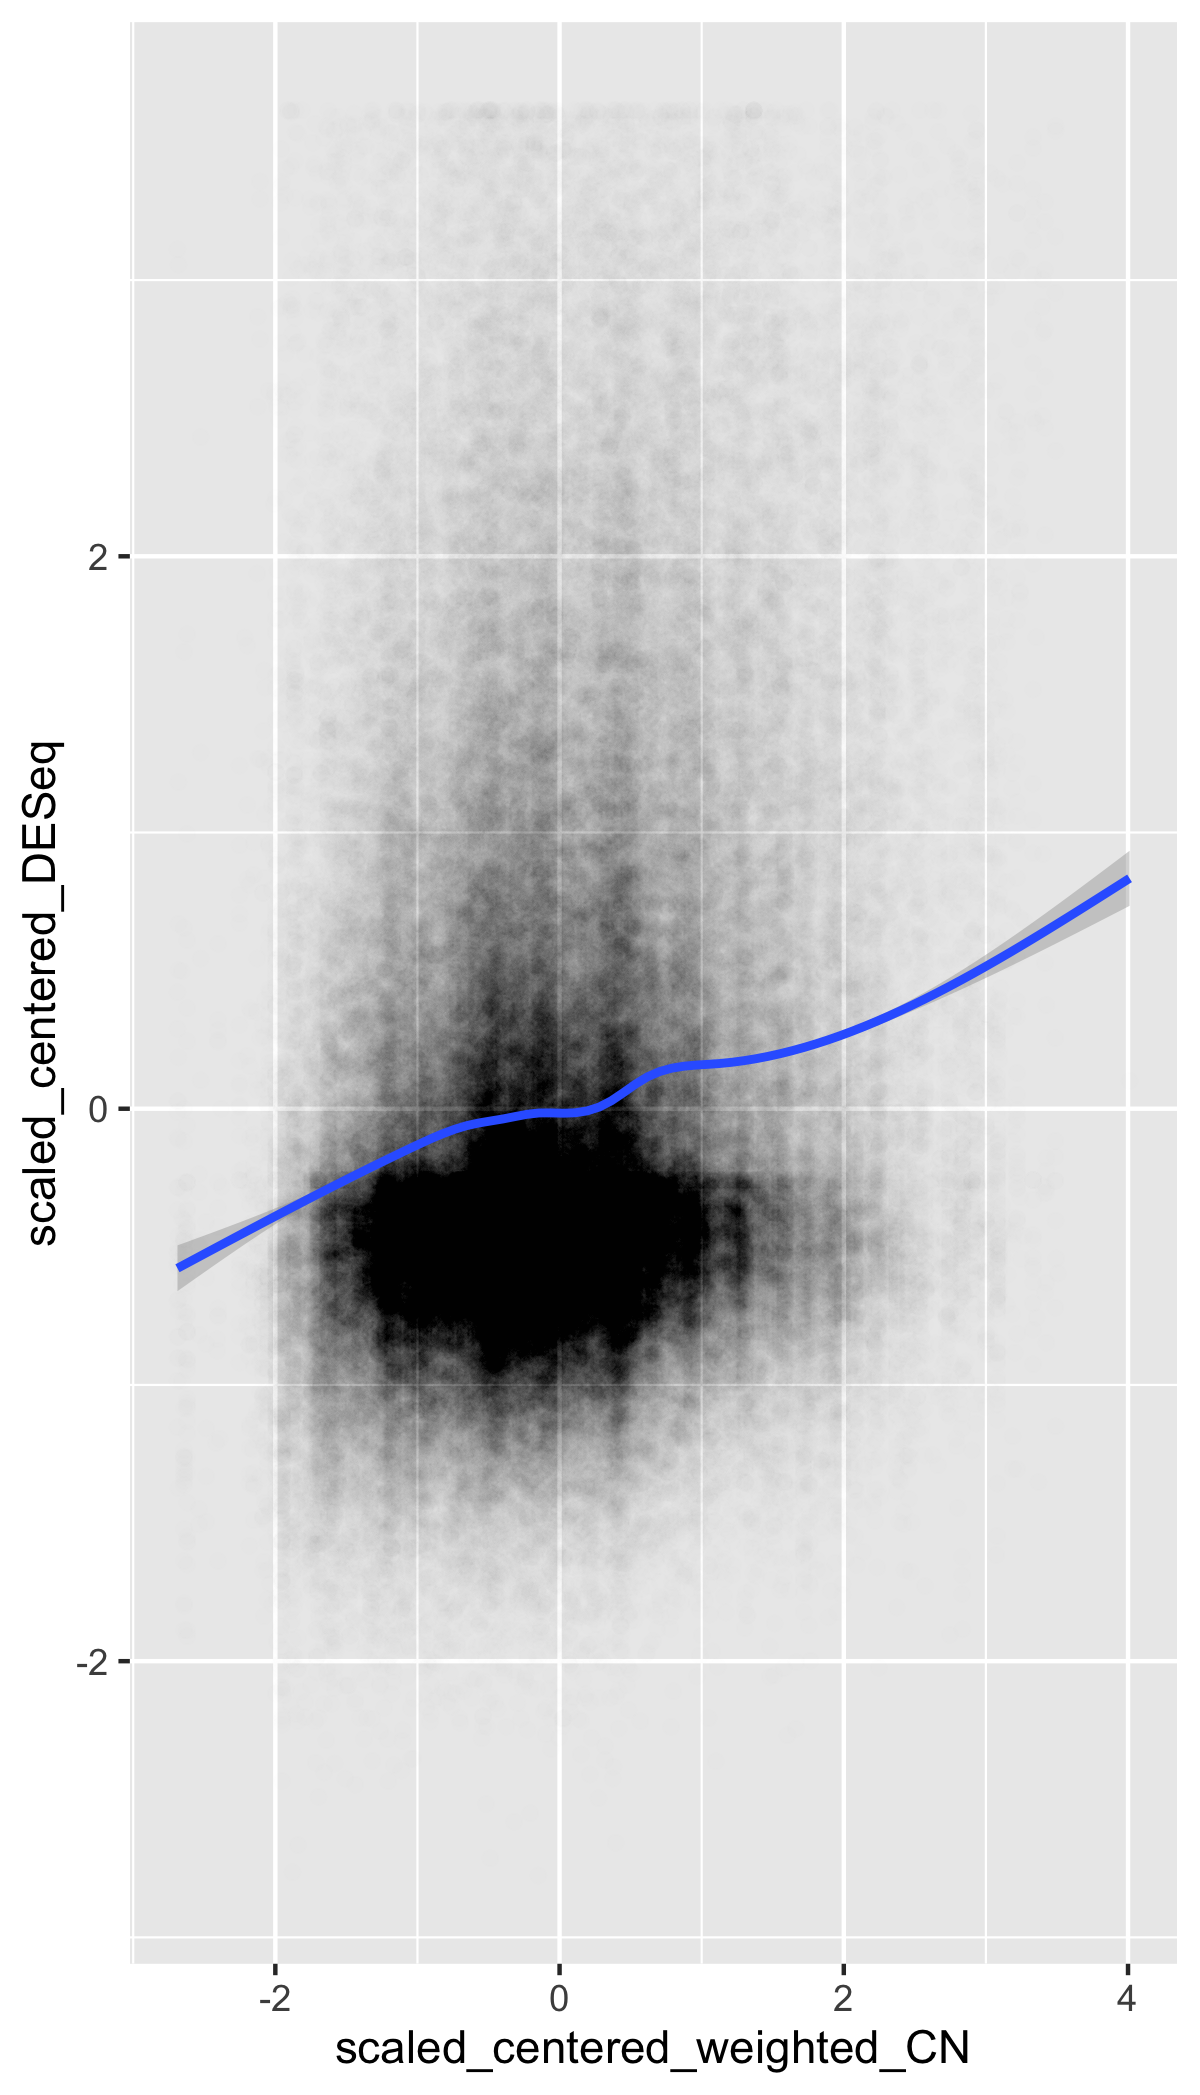
\includegraphics[width=1.7in]{../../RNASeq_and_CN/figures/scatterplot_normCNweighted_normDESeq_nonormal.png}
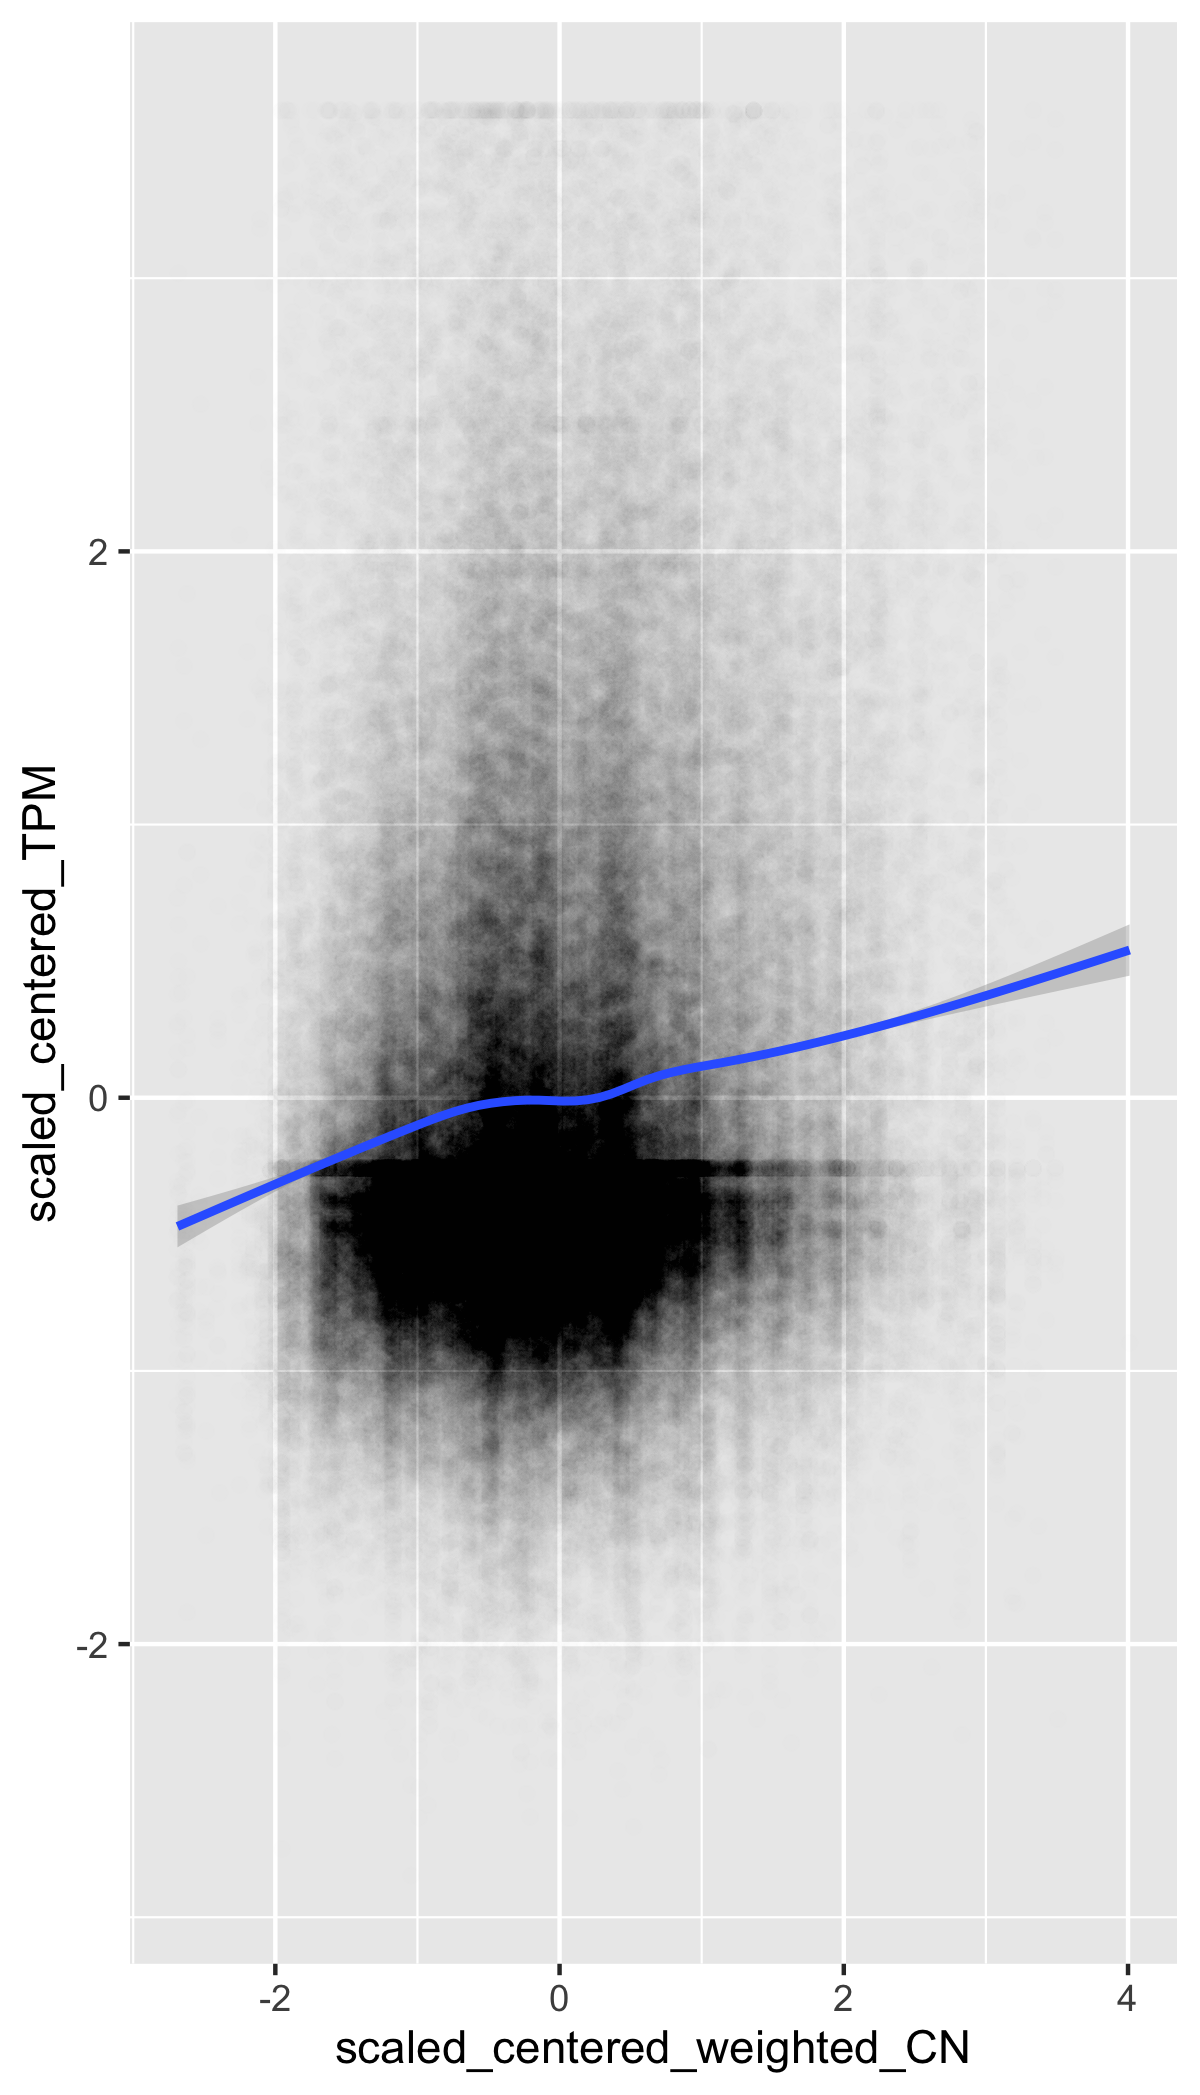
\includegraphics[width=1.7in]{../../RNASeq_and_CN/figures/scatterplot_normCNweighted_normTPM_nonormal.png}
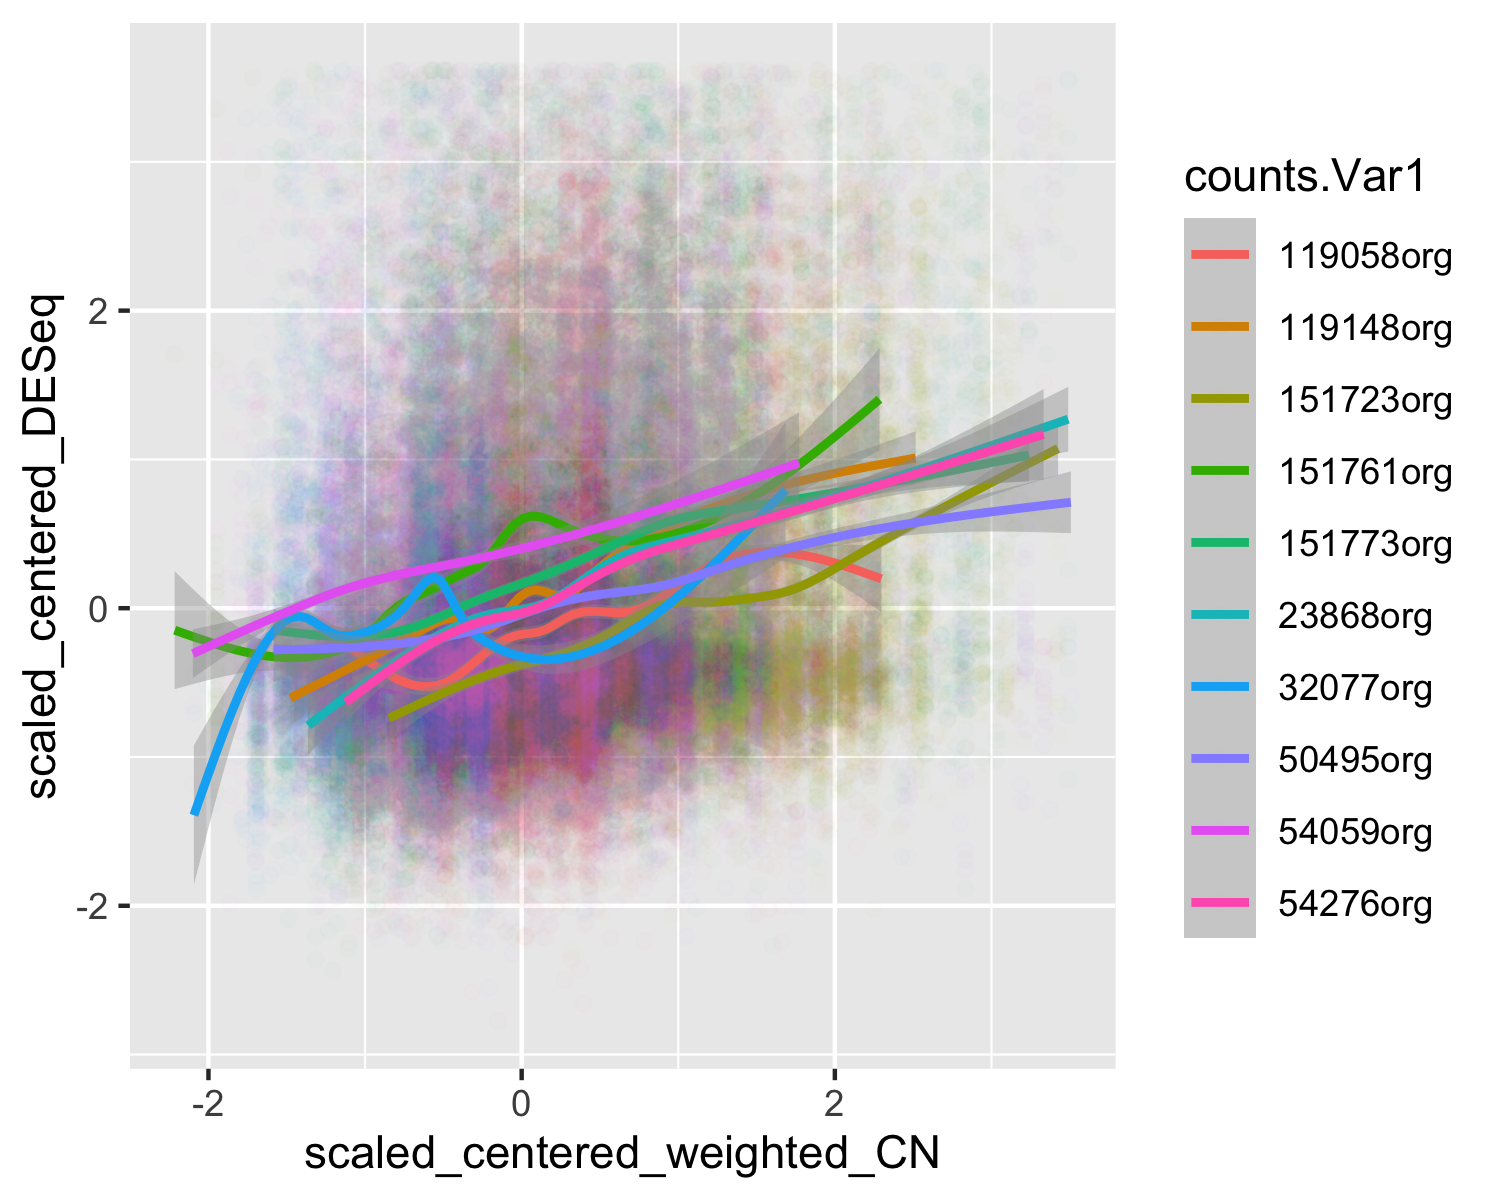
\includegraphics[width=2.8in]{../../RNASeq_and_CN/figures/scatterplot_normCNweighted_normDESeq_perorg2_subsetorgs.png}\\
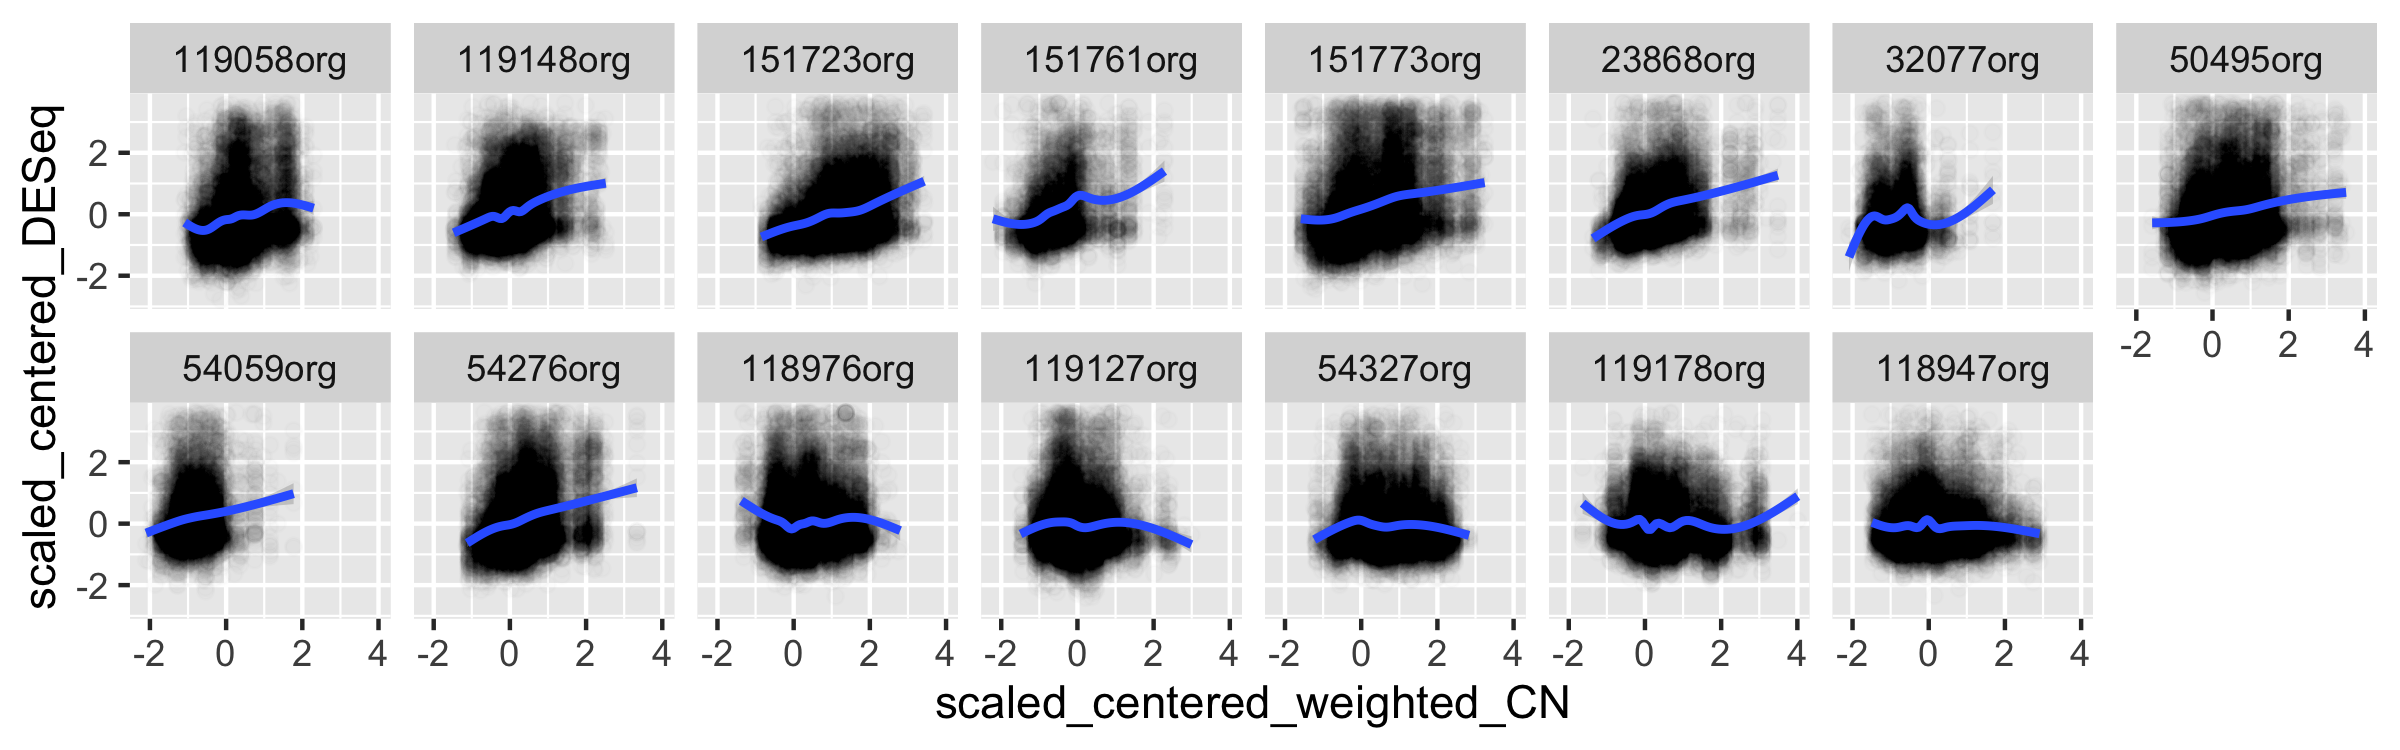
\includegraphics[width=\textwidth]{../../RNASeq_and_CN/figures/scatterplot_normCNweighted_normDESeq_perorg2.png}
%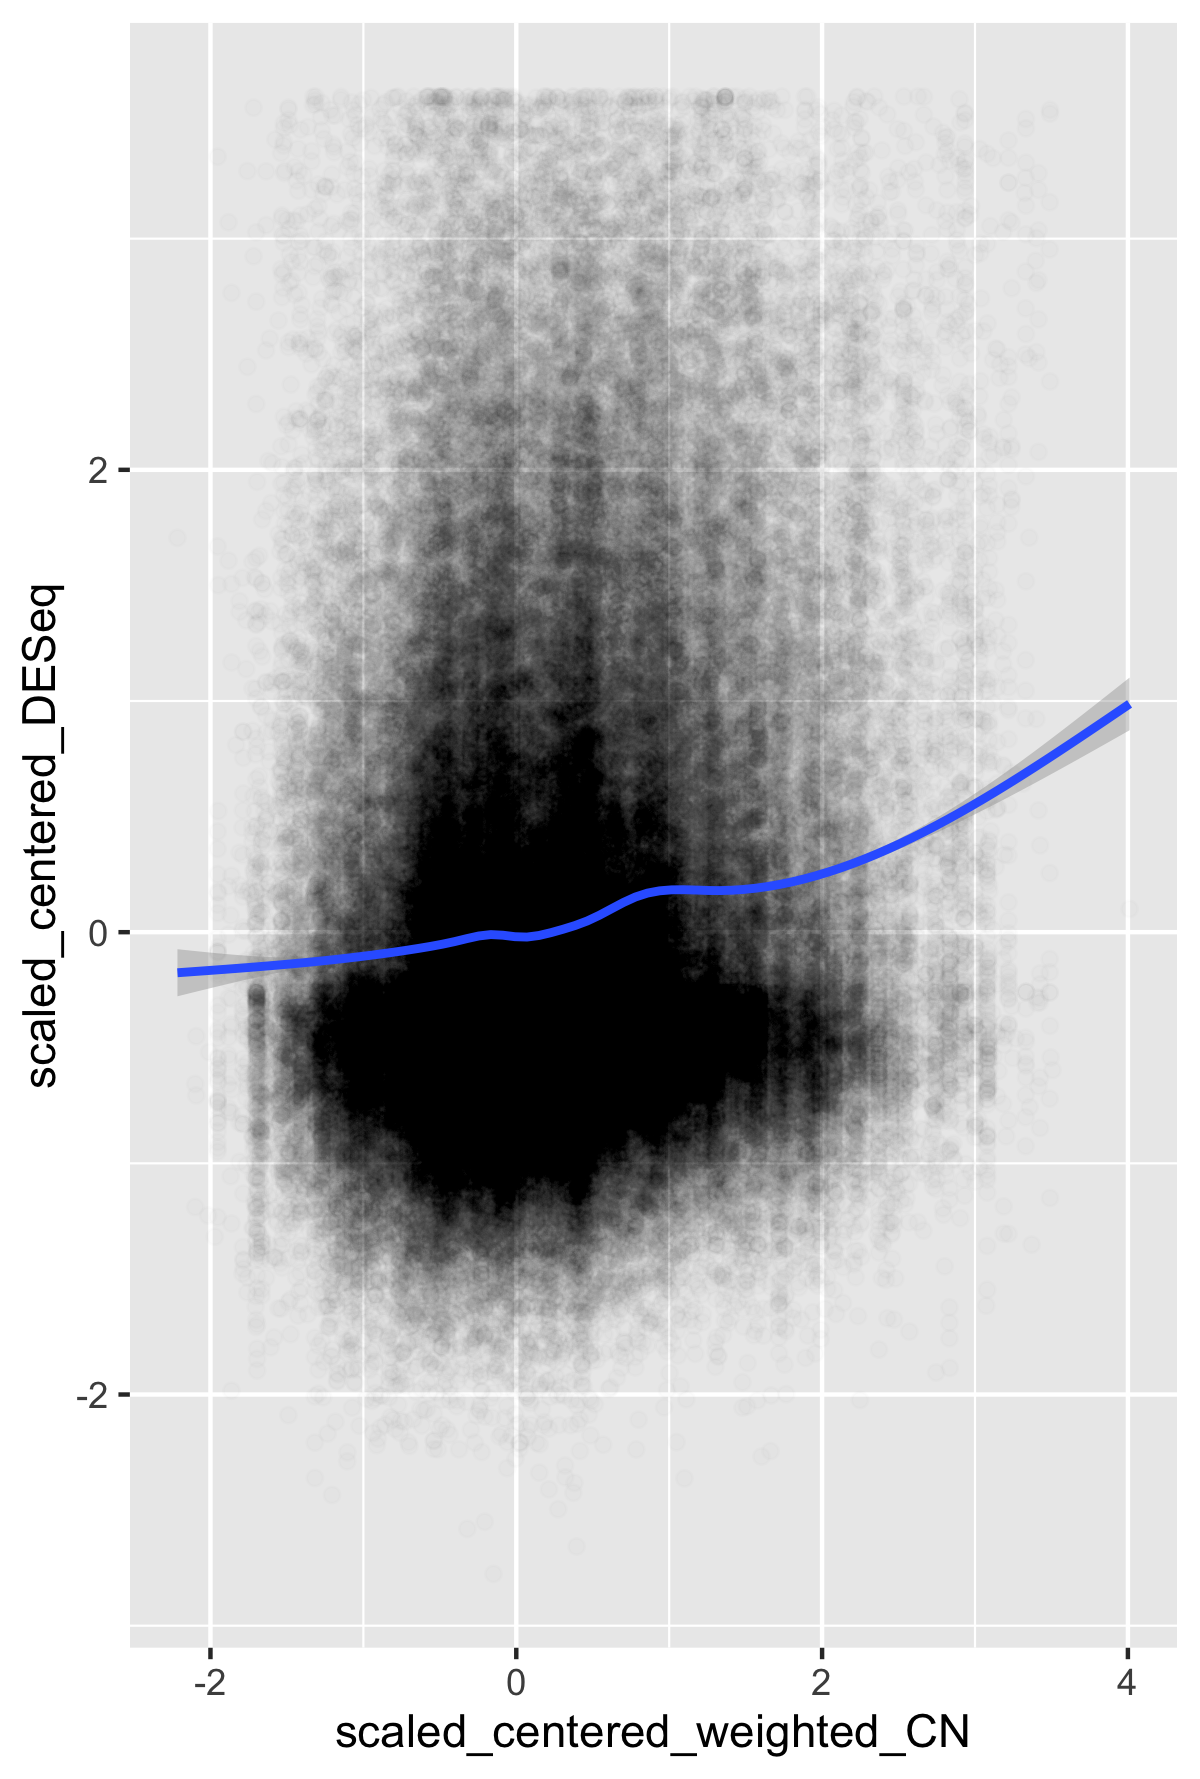
\includegraphics[width=1.7in]{../../RNASeq_and_CN/figures/scatterplot_normCNweighted_normDESeq_nonormal_onlyamp.png}
\caption{Scaled and centered CN and GE (DESeq2 and TPM respectively). Right: same, color-coded per organoid, but only for organoids which show a positive trend between CN and GE. Below: split per organoid. The same results are found when normal segments are kept. \label{fig:scaled_CN_GE}} %When only looking at amplifications (third plot; for DESeq2 counts) the trend is even clearer}
\end{figure}


\begin{figure}[h]
\centering
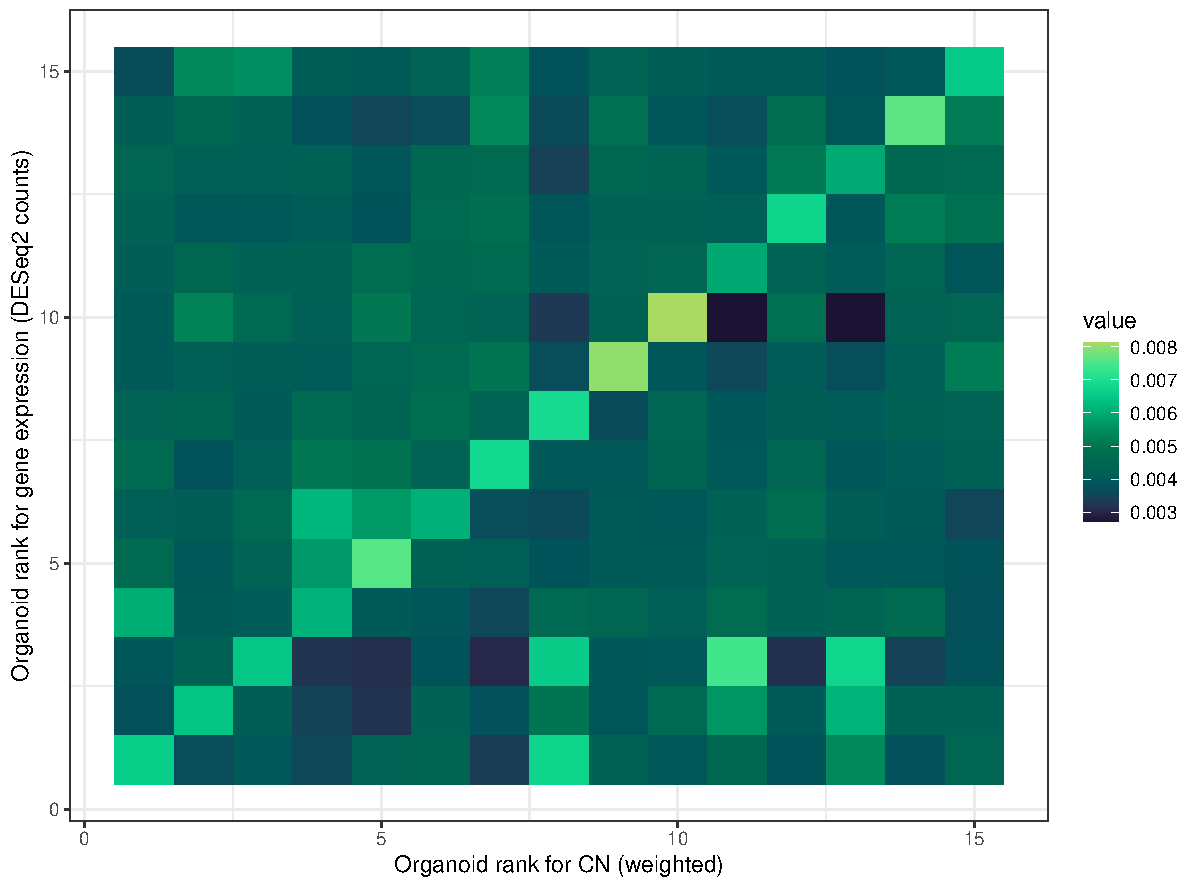
\includegraphics[width=3in]{../../RNASeq_and_CN/figures/rankplot_CNweighted_deseq.pdf}
\caption{Normalised matrix of ranks. I.e., for each gene, the organoid samples are ranked by CN and GE,  independently,  in ascending order. The correlation between these two ranks can be seen as a matrix that contains 15 entries of value 1 (one for each column and each row), and in which all other entries are zero. If there is a complete agreement between the ranks of GE and CN, we have a diagonal matrix (entries of 1 in the diagonal, and of 0 in the off-diagonal). This procedure is repeated for each gene. Then all the matrices are added together to give a matrix of counts. The sum of all entries is the number of organoids (15) times the number of genes. This matrix is then normalised by this number, so that the entries add up to one, which is plotted here. A bright diagonal indicates a very good agreement between the rank of GE and rank of CN across organoids.\label{fig:rank_CN_GE} The off-diagonal entries at GE ranks 1 and 2 indicate that there are many genes for which the rank of CN is high (high copy number, relative to other organoids) but the rank of GE is low (low gene expression values, relative to other organoids).}
\end{figure}

\medskip

If we ask the question of whether genes which are in highly amplified regions have a higher gene expression than the same gene in normal fallopian tissue (average over five fallopian samples of healthy patients) the answer is overwhelmingly \emph{not} (102174 sample/genes combinations for which it's not the case,  64621 for which it is, when the copy number is higher than 2), with most genes having actually lower expression values than normal tissue. This is confounded by compositionality/ assuming that most genes remain the same. Moreover, the normal samples don't come from the same patients as the organoids.

\clearpage
\subsection{Correlation of specific genes}
After the genome-wide analyses of the previous section, here we focus on the genes of interest, and the genes that show the highest correlation between copy number and gene expression. Figure~\ref{cn_ge_specific_genes} shows all the results. I explain the plots below:

\paragraph{Row 1, Column 1} For each gene of interest (x axis) we plot their copy number (y) axis, for all organoids, as a violin plot. We also add the values of each organoid as points. The colour of each point is the scaled and centered gene expression value. If there was a correlation between CN and GE we would expect to see a gradient of colours as the copy number increases, within each gene, which we don't see. The grey lines connect observations from the same organoid. As there are grey lines everywhere, it means that there is no general trend of any organoid having consistently higher or lower copy number than the others. Perhaps there is an exception in the top-CN organoids in genes ATM, TUBB1, TOP1.

\paragraph{Row 1, Column 2} Same as the previous plot, but this time the y axis indicates the GE values, and the colour is the CN.

\paragraph{Row 2, Column 1} For all genes, we have computed two metrics of agreement between CN and GE. On the y axis, we have the $R^2$ of the linear relationship between the two. On the x axis, I have the comparison of the GE of high-CN organoids to the GE of low-CN organoids. In particular, I have computed the mean DESeq2 count for the three organoids of lowest CN, and compared the DESeq2 counts of the remaining organoids (of higher CN), for each gene independently. The genes at the top right of the plot are genes which show good GE-CN agreement according to both metrics. The labels indicate genes of interest, out of which only AKT2 shows a decent agreement between GE and CN. The boxplots show the summary of genes that share the same second metric (which is discrete as it's a fraction of organoids, out of 13 organoids, and therefore can take 13 different values).

\paragraph{Row 2, Column 2} Same as previous plot, but this time the labels are for genes at the upper-right hand corner.

\paragraph{Row 3, Column 1} Example of a gene at the the upper-right hand corner. The trend is driven by a single organoid. This is the case for many genes.

\paragraph{Row 3, Column 2} Genes sorted by the second metric of agreement (same as in x axis of figure in Row 2, Column 1). A value of 0.5 indicates that half of the high-CN organoids have a GE lower than the mean GE of low-CN organoids, and half have a higher GE, for some gene. The labels are for genes of interest. Most of them are on the upper half of the plot, indicating some positive trend between GE and CN, with the exception of MECOM and TERT, and some genes at 0.5.

\begin{figure}[h]
\centering
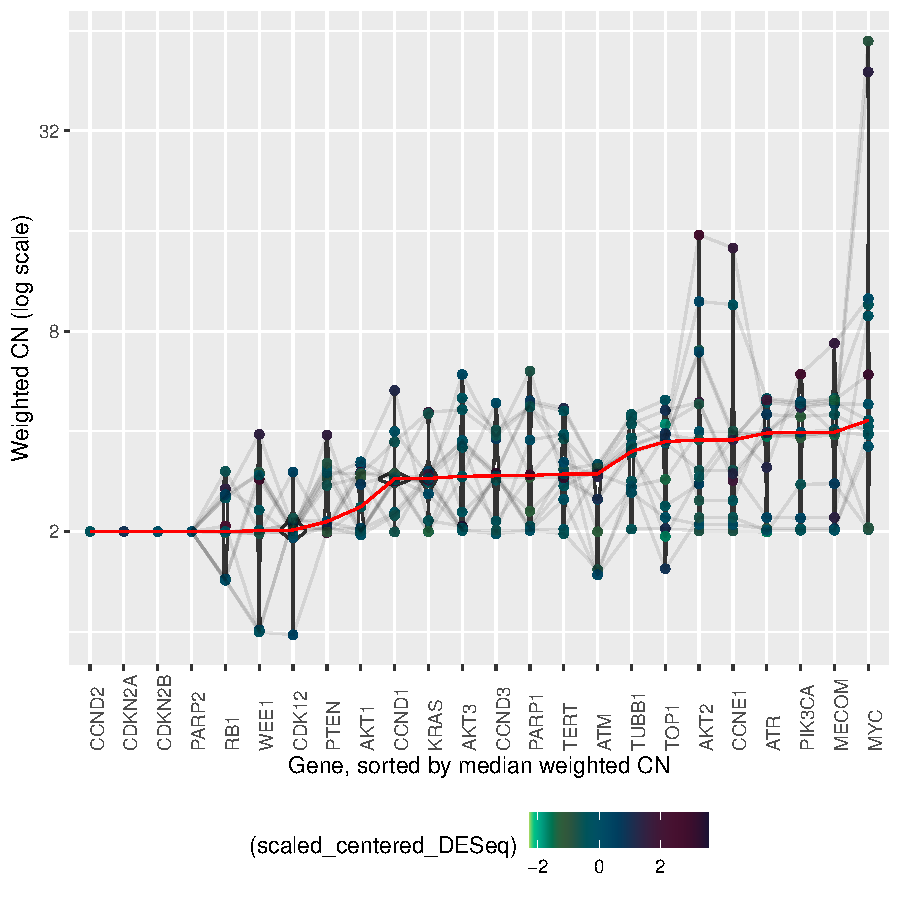
\includegraphics[width=.45\textwidth]{../../RNASeq_and_CN/figures/CN_violinplots_goi.pdf}
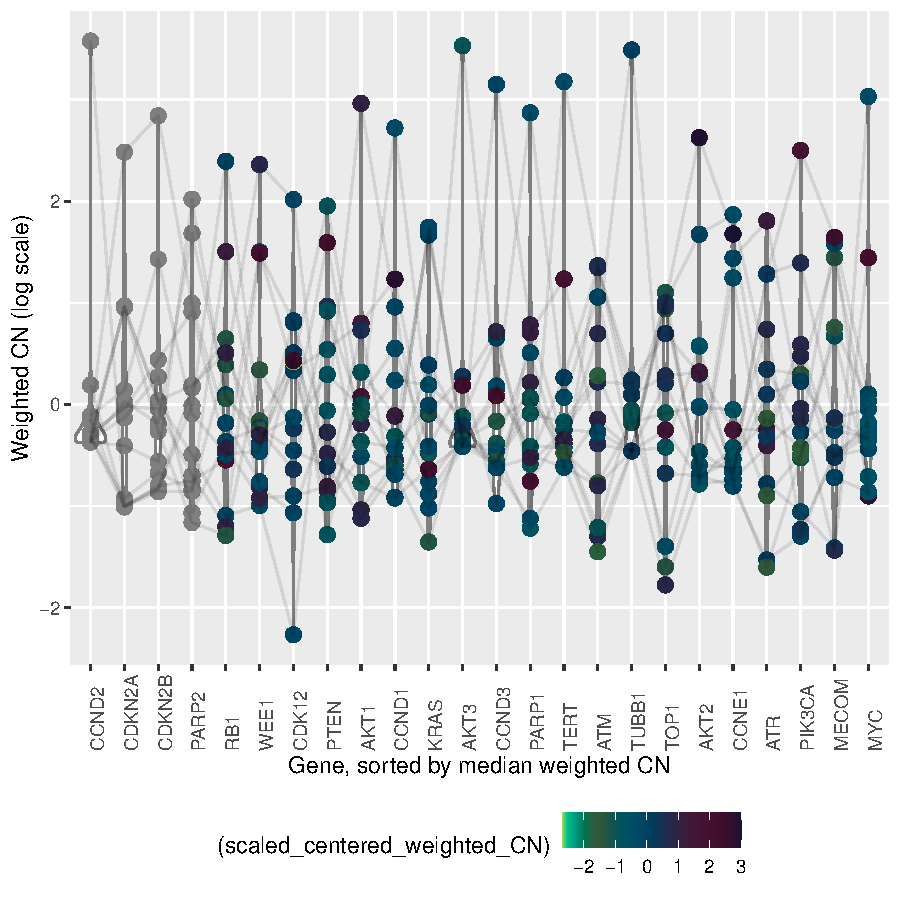
\includegraphics[width=.45\textwidth]{../../RNASeq_and_CN/figures/CN_violinplots_goi_2.pdf}
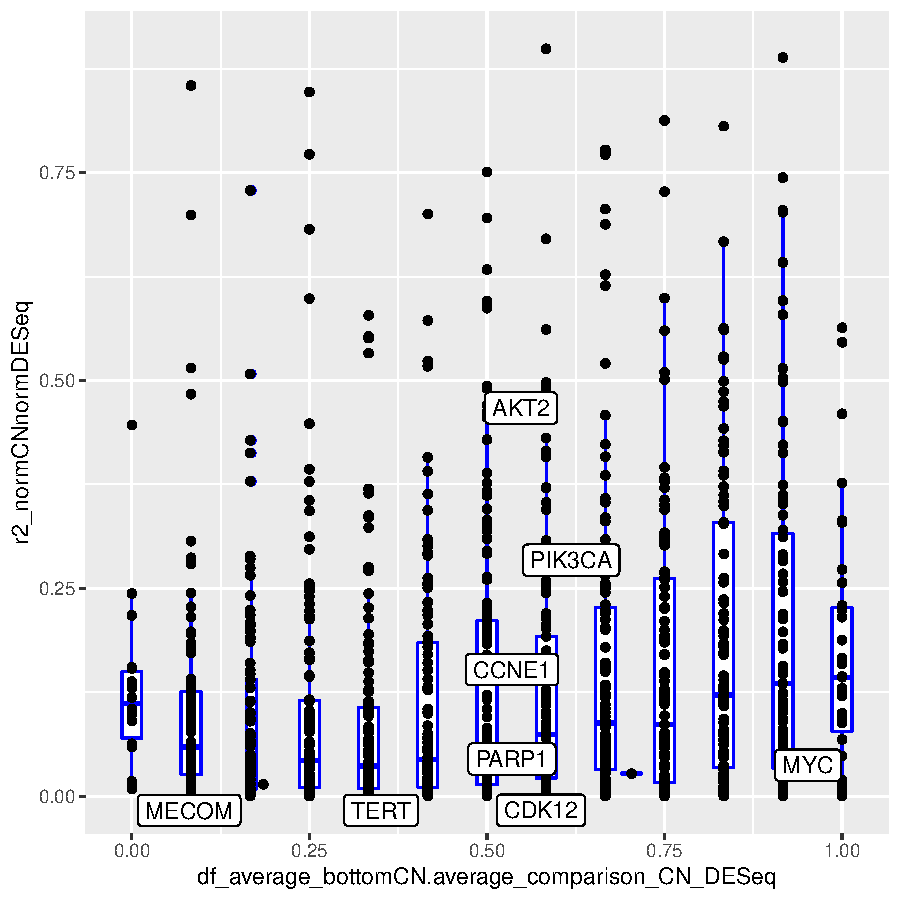
\includegraphics[width=3in]{../../RNASeq_and_CN/figures/r2normCNnormDESeq_vs_averagebottomCN.pdf}
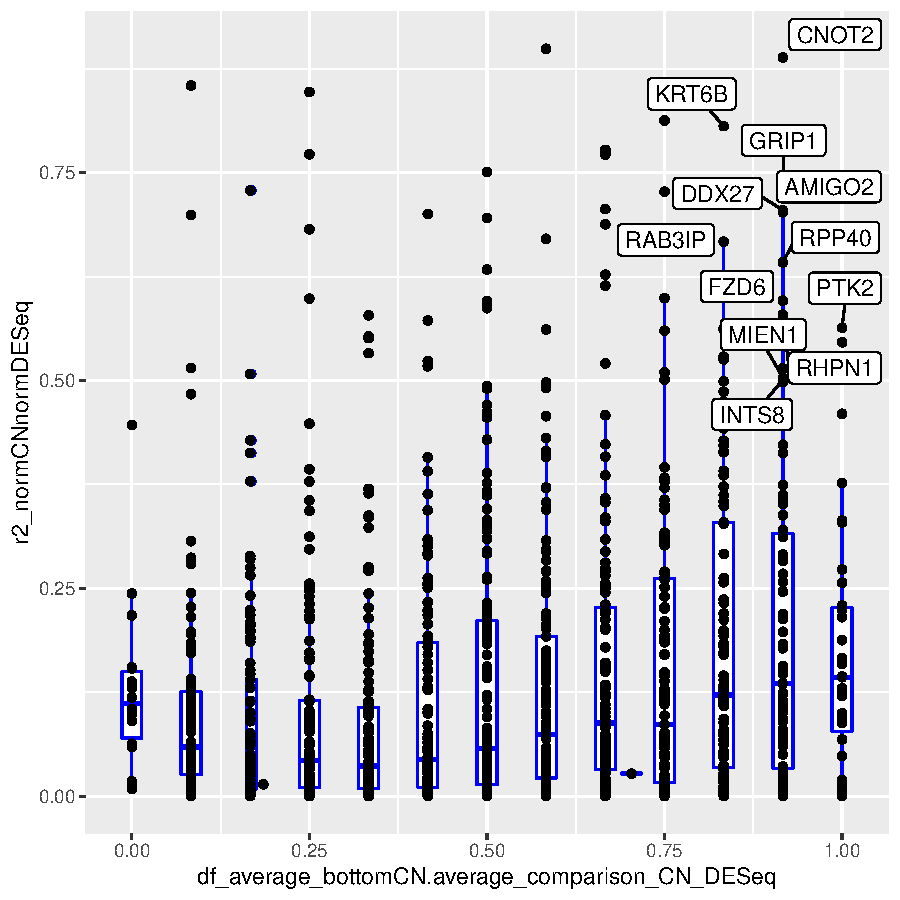
\includegraphics[width=3in]{../../RNASeq_and_CN/figures/r2normCNnormDESeq_vs_averagebottomCN_best.pdf}
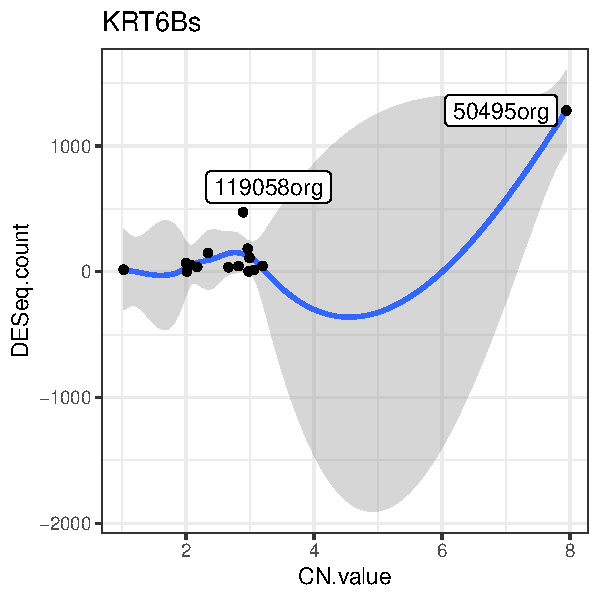
\includegraphics[width=2.5in]{../../RNASeq_and_CN/figures/example_KRT6B.pdf}
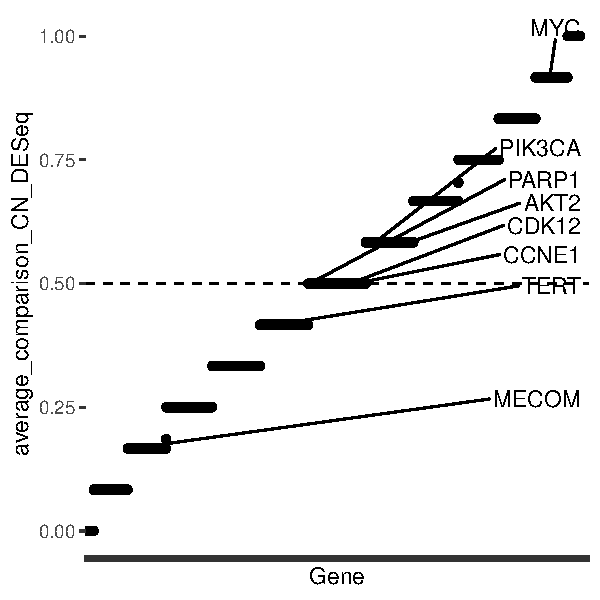
\includegraphics[width=3in]{../../RNASeq_and_CN/figures/average_bottomCN_DESeq.pdf}
\caption{Fraction of samples with gene expression higher than the bottom three samples of lowest copy number. Higher values indicate a correlation between copy number and gene expression.\label{cn_ge_specific_genes}}
\end{figure}

\end{document}